%==========================================================================
\chapter{Example of Figure Use}
\label{Example of Figure Use}

Here is an example of how figures might be used.  Here we want to
illustrate how a figure is included in both the printed manual and the
online manual.  So, see Figure \ref{fig-conceptual-interface}.  The
\code{figure} environment is automatically converted to a GIF image by
LaTeX2HTML, so graphics included this way need only exist in
postscript format.  Note that the conversion loses the colors at the
moment, but I am assured that this can be fixed.
\begin{figure}
\centering
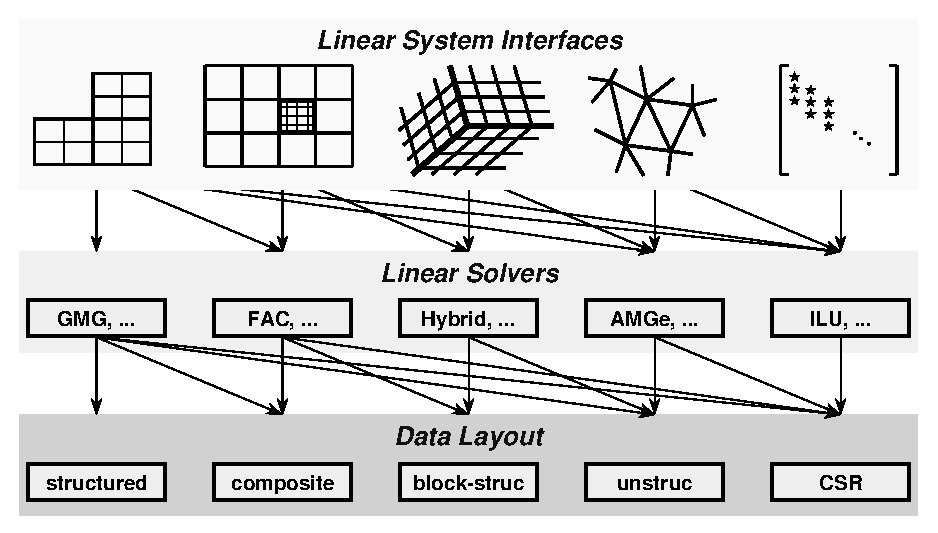
\includegraphics[width=5in]{concep_iface.ps}
\caption{%
Graphic illustrating the notion of conceptual interfaces.}
\label{fig-conceptual-interface}
\end{figure}

To insert graphics that are not figures (i.e., not in a figure
environment), where both a \code{.ps} and a\code{.gif} file have
already been created, use the macro \code{InsertGraphics}.  This
produces the following:

\begin{center}
\InsertGraphics{concep_iface}{width=5in}
\end{center}
